\documentclass[11pt, a4paper]{article}

% --- Essential Packages ---
\usepackage[utf8]{inputenc}    % Text encoding
\usepackage{graphicx}          % Required for inserting images
\usepackage{url}               % Required for robust URL handling
\usepackage{hyperref}          % Required for links and URLs
\usepackage{geometry}          % Adjust page margins
\geometry{margin=2.5cm}

% --- Document Information ---
\title{\textbf{Labwork 5 Report: Gaussian Blur Convolution}}
\author{Lucien Elyas Bedrane \\ Student ID: 2640012}
\date{\today}

\begin{document}

\maketitle

% --- Section 1: Objective Breakdown ---
\section{Objectives \& Breakdown}
This lab is a continuation of labwork 4 where we modify our previous work in order to use the 7x7 Gaussian Blur Convolution with our CPU and GPU with and without shared memory.

% --- Section 2: Code Output Image ---
\section{Implementations \& Results}
First, I implemented the mathematical formula seen in the course to create the Gaussian mask using the get\_gaussian\_kernel() function. This function calculates the weights of a 7x7 matrix based on the Gaussian distribution equation, where the weights naturally decrease as we move further away from the center coordinates.
\\Using this mask, I developed the CPU version of the Gaussian blur gaussian\_blur\_CPU(). The logic operates by sliding the 7x7 kernel over every pixel of the image, deliberately excluding the borders to avoid out-of-bounds errors. For each color channel of a target pixel, the algorithm iterates through its 49 neighboring pixels. It multiplies each neighbor's value by the corresponding weight in the Gaussian mask, and sums these values to compute the new blurred pixel. This exact sliding-window logic is the foundation that we apply to the GPU versions.
\\For the GPU implementation without shared memory, I reused the grid and block coordinate structure from the Grayscale kernel we made in Labwork 4. I simply replaced the grayscale conversion mathematics with the nested loops we implemented in the CPU version. In this version, every thread reads the image pixels and the kernel weights directly from the global memory for every calculation.
\\For the GPU version with shared memory, the objective is to optimize memory access. Since the 7x7 kernel is strictly identical for every thread, we load it into the GPU's shared memory at the beginning of the block execution. A critical detail here concerns thread synchronization. The course material illustrated block synchronization using cuda.synchronize() inside the function. However, doing so makes the code crash. According to the official NVIDIA CUDA and Numba documentation, cuda.synchronize() is the host-side command used to make the CPU wait for the GPU. Therefore, to correctly synchronize threads within the same block on the device, we must use cuda.syncthreads().
\clearpage
Once the implementations were complete, I generated a graph to plot the Speedup (CPU time divided by GPU time) against the Block Size that we can see bellow :
 
\begin{figure}[h!]
    \centering
    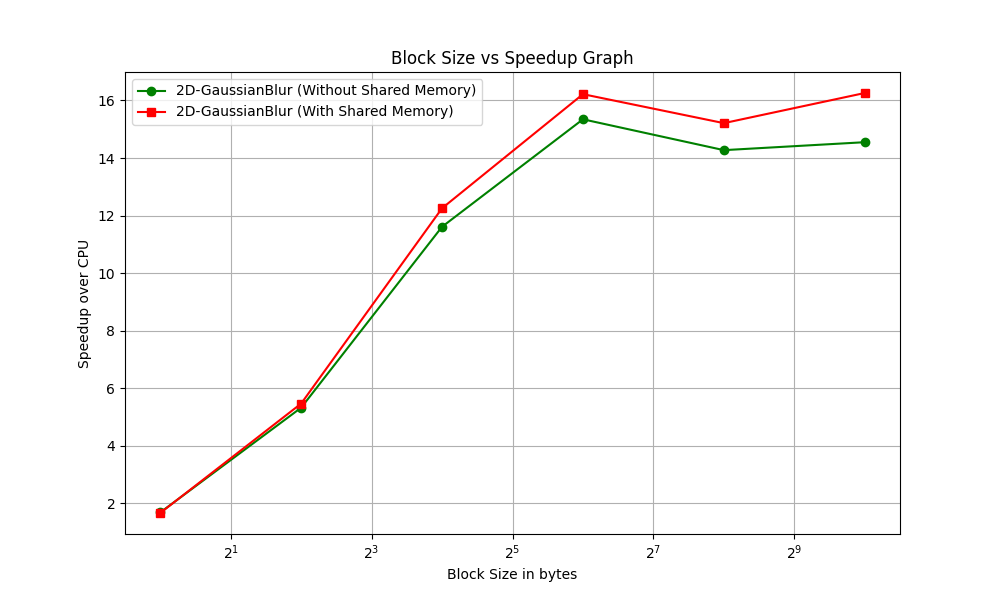
\includegraphics[width=0.8\textwidth]{plots/BlockSize_vs_Speedup_Graph} 
    \caption{Block size vs Speedup graph.}
    \label{fig:graph}
\end{figure}

As we can see in the graph, at small block sizes, the speedup is relatively low as we do not make use of the capacity of the GPU for parralelization calculations. The higher the block sizes, the better the GPU verions outperforms the CPU we an increase of ~16x in performance. When we compare both implementations of the GPU versions, we can see that the shared memory version is slightly better than the one that doesn't utilize it for high block sizes.
\\Lastly, as a small comment, I applied the @numba.jit decorator to the CPU version of the Gaussian Blur. I had to use this compilation command because testing the algorithm on my very large image (7680x4320 pixels) using pure Python loops did not finish even after running for more than 35 minutes. By compiling the CPU baseline with JIT to achieve native C-speed execution, it only took 218 seconds for the entire program to run (including all the GPU versions and image saving steps), providing a fair and realistic sequential baseline for our speedup calculations.

% --- Section 3: Sources ---
\section{Sources \& References}
The following resources and documentation were used to complete this work:

\begin{itemize}
    \item Thread and Memory Model by Tran Giang Son for M2 at ICT\\
    \item Numba guide for syncthreads \\
    \url{https://numba.readthedocs.io/en/stable/cuda-reference/kernel.html?highlight=syncthr#numba.cuda.syncthreads}
\end{itemize}

\end{document}
